%%%%%%%%%%%%%%%%%%%%%%%%%%%%%%%%%%%%%%%%%%%%%%%%%%%%%%%%%%%%%%%%%%%%%%%%%%%%%%%
% Preamble
%%%%%%%%%%%%%%%%%%%%%%%%%%%%%%%%%%%%%%%%%%%%%%%%%%%%%%%%%%%%%%%%%%%%%%%%%%%%%%%
\documentclass[aspectratio=169]{beamer}

% Packages
\usepackage{amsthm}
\usepackage{amssymb}
\usepackage{amsfonts}
\usepackage{amsmath}
\usepackage{mathtools}
\usepackage{pgf}
\usepgflibrary{fpu}
\usepackage{pgfplots}
\usepackage{tikz}
\usetikzlibrary{angles,fit,arrows,calc,math,matrix,intersections,through,backgrounds}
\usepackage{tikz-cd}
\usepackage{tkz-euclide}
\usepackage{tkz-graph}
\usepackage{graphicx}
\usepackage{hyperref}
\pgfplotsset{compat=1.18}

% Theme
\usetheme{Pittsburgh}
\usecolortheme{seahorse}

% Title and Author
\title{Arithmetic Expression Geometry:\\Five Possibilities}
\author[Mingli Yuan]{Mingli Yuan}
\date{\today}

\begin{document}

%%%%%%%%%%%%%%%%%%%%%%%%%%%%%%%%%%%%%%%%%%%%%%%%%%%%%%%%%%%%%%%%%%%%%%%%%%%%%%%
% Title and Introduction
%%%%%%%%%%%%%%%%%%%%%%%%%%%%%%%%%%%%%%%%%%%%%%%%%%%%%%%%%%%%%%%%%%%%%%%%%%%%%%%

\begin{frame}
    \maketitle
\end{frame}

\begin{frame}
    \frametitle{Table of Contents}
    \tableofcontents
\end{frame}

%%%%%%%%%%%%%%%%%%%%%%%%%%%%%%%%%%%%%%%%%%%%%%%%%%%%%%%%%%%%%%%%%%%%%%%%%%%%%%%
%
%%%%%%%%%%%%%%%%%%%%%%%%%%%%%%%%%%%%%%%%%%%%%%%%%%%%%%%%%%%%%%%%%%%%%%%%%%%%%%%

\section{Foreword: A few small, colorful stones}

\begin{frame}
    \frametitle{Foreword: A few small, colorful stones}
        \begin{columns}
        \begin{column}{0.55\textwidth}
Over the past ten years of exploration, I’ve collected a few small, colorful stones.
\newline\newline
Each one sparked my curiosity, and together they have carried me to where I am today.
\newline\newline
The stones are not answers, but invitations — to keep exploring, to keep asking.
        \end{column}
        \begin{column}{0.45\textwidth}
            \begin{figure}[ht]\centering
                \resizebox{0.7\textwidth}{!}{\includegraphics{../images/rock_balancing}}
            \end{figure}
        \end{column}
    \end{columns}

\end{frame}

%%%%%%%%%%%%%%%%%%%%%%%%%%%%%%%%%%%%%%%%%%%%%%%%%%%%%%%%%%%%%%%%%%%%%%%%%%%%%%%
% Possibility 1: From Non-commutativity to Complexity
%%%%%%%%%%%%%%%%%%%%%%%%%%%%%%%%%%%%%%%%%%%%%%%%%%%%%%%%%%%%%%%%%%%%%%%%%%%%%%%

\section{Ochre: The red stone of beginnings}

\begin{frame}
    \frametitle{Ochre: The red stone of beginnings}
    \begin{center}
        \Large
        \textbf{From Non-commutativity to Complexity}\newline\newline
        \emph{How does non-commutativity lead to complexity, and how can we geometrize it?}
    \end{center}
\end{frame}

\begin{frame}
\frametitle{Regularity of word2vec}
A well-known example is word2vec:

\begin{itemize}
    \item Parallelism encodes semantic analogy: concepts are points, relations are vectors.
    \item However, this regularity is not fully or rigorously enforced in word2vec. What happens if we enforce it strictly?
\end{itemize}
\begin{figure}[ht]
\centering
\resizebox{0.5\textwidth}{!}{
\begin{tikzpicture}[x=0.5cm,y=0.5cm,z=0.3cm,>=stealth]
\draw[->] (xyz cs:x=-7.0) -- (xyz cs:x=7.0) node[above] {$x_0$};
\draw[->] (xyz cs:y=0) -- (xyz cs:y=7.0) node[right] {$x_n$};
\draw[->] (xyz cs:z=-7.0) -- (xyz cs:z=7.0) node[above] {$x_i$};

\node[fill,circle,inner sep=1.5pt,label={left:$king$}] (p) at (xyz cs:x=-3.0, y=3.0, z=-3.0) {};
\node[fill,circle,inner sep=1.5pt,label={right:$man$}] (q) at (xyz cs:x=2.0, y=-3.0, z=3.0) {};
\node[fill,circle,inner sep=1.5pt,label={left:$queen$}] (r) at (xyz cs:x=-3.0, y=3.0, z=3.0) {};
\node[fill,circle,inner sep=1.5pt,label={right:$woman$}] (s) at (xyz cs:x=2.0, y=-3.0, z=9.0) {};
\draw[dashed, blue] (p) -- (q);
\draw[dashed, blue] (r) -- (s);
\draw[dashed, red] (p) -- (r);
\draw[dashed, red] (q) -- (s);
\end{tikzpicture}
}
\caption{Regularity in word2vec}
\label{fig:regularity-of-word2vec}
\end{figure}
\end{frame}

\begin{frame}
\frametitle{The case of numbers}
\[
(\alpha + 1) \times 2 \neq \alpha \times 2 + 1
\]

\begin{itemize}
    \item First-class elements: numbers (points), operations (generators), and relationships (operation sequences/paths) are modeled explicitly.
    \item Regularity strictly enforced: the same operation sequence induces the same geometric displacement; different orders encode different relationships.
    \item Both ``relationship'' and ``concept'' are treated as first-class, fully consistent with this regularity.
\end{itemize}

\begin{figure}[ht]
\centering
\resizebox{0.5\textwidth}{!}{
\begin{tikzpicture}[x=0.5cm,y=0.5cm,z=0.3cm,>=stealth]
\draw[->] (xyz cs:x=-7.0) -- (xyz cs:x=7.0) node[right] {$x_0$};
\draw[->] (xyz cs:y=0) -- (xyz cs:y=7.0) node[right] {$x_n$};
\draw[->] (xyz cs:z=-7.0) -- (xyz cs:z=7.0) node[above] {$x_i$};

\node[fill,circle,inner sep=1.5pt,label={left:$\alpha$}] (p) at (xyz cs:x=-3.0, y=3.0, z=-3.0) {};
\node[fill,circle,inner sep=1.5pt,label={right:$\alpha+1$}] (q) at (xyz cs:x=2.0, y=-3.0, z=3.0) {};
\node[fill,circle,inner sep=1.5pt,label={left:$\alpha \times 2$}] (r) at (xyz cs:x=-3.0, y=3.0, z=3.0) {};
\node[fill,circle,inner sep=1.5pt,label={right:$(\alpha + 1) \times 2 \neq \alpha \times 2 + 1$}] (s) at (xyz cs:x=2.0, y=-3.0, z=9.0) {};
\draw[dashed, blue] (p) -- (q);
\draw[dashed, blue] (r) -- (s);
\draw[dashed, red] (p) -- (r);
\draw[dashed, red] (q) -- (s);
\end{tikzpicture}
}
\caption{Non-commutativity of operations in Euclidean space}
\label{fig:noncommutativity-numbers}
\end{figure}
\end{frame}

\begin{frame}
    \frametitle{Explosion of symbolic combinations}
    \begin{columns}
        \begin{column}{0.55\textwidth}
            \begin{itemize}
                \item Once non-commutativity is introduced, the number of distinct operation strings grows \emph{exponentially}.
                \item Generation trees visualize this explosion: greater depth leads to a combinatorial surge in distinct expressions.
                \item Intuition: branching factor $>1$ implies exponential growth.
            \end{itemize}
        \end{column}
        \begin{column}{0.45\textwidth}
            \begin{figure}[ht]\centering
                \resizebox{0.9\textwidth}{!}{\includegraphics{../images/explosion}}
                \caption{Tree expansion of possible generation sequences}
            \end{figure}
        \end{column}
    \end{columns}
\end{frame}

\begin{frame}
    \frametitle{From symbols to geometry: hyperbolicity and volume}
    \begin{itemize}
        \item Assume each operation sequence maps to a point in a geometric space, and that balls of radius $\delta$ have uniformly positive volume.
        \item Then the symbolic explosion caused by non-commutativity corresponds to exponential growth of volume.
        \item Hyperbolic spaces exemplify this behavior:
        \[
            \mathrm{Vol}(B_r) \sim e^{(n-1)r}
        \]
    \end{itemize}
    \begin{columns}
        \begin{column}{0.3\textwidth}
            \begin{figure}[ht]\centering
                \resizebox{0.9\textwidth}{!}{\includegraphics{../images/non-parallelogram}}
                \caption{Non-parallelogram $\Rightarrow$ hyperbolicity}
            \end{figure}
        \end{column}
        \begin{column}{0.3\textwidth}
            \begin{figure}[ht]\centering
                \resizebox{0.5\textwidth}{!}{\includegraphics{../images/t4096}}
                \caption{A hyperbolic tessellation}
            \end{figure}
        \end{column}
    \end{columns}
\end{frame}

\begin{frame}
    \frametitle{Contrast: the linear/commutative case}
    \begin{itemize}
        \item If operations commute or are constrained by linearity, the \emph{parallelogram law} holds.
        \item The parallelogram law simplifies the generation process and mitigates the explosion of symbolic combinations.
        \item Euclidean ball volume: $\mathrm{Vol}(B_r) \propto r^n$ (polynomial in $r$).
    \end{itemize}
    \begin{figure}[ht]\centering
        \resizebox{0.5\textwidth}{!}{\includegraphics{../images/parallelogram}}
        \caption{Parallelogram law $\Rightarrow$ Euclidean linearity}
    \end{figure}
\end{frame}

\begin{frame}
    \frametitle{Conclusion: complexity as a geometric volume}
    We have shown that:
    \begin{itemize}
        \item Commutativity implies the parallelogram law and Euclidean linearity.
        \item In the commutative (linear) case, volumes grow polynomially: Euclidean space.
        \item Non-commutativity breaks the parallelogram law, yielding exponential growth: hyperbolic space.
    \end{itemize}
    More broadly, geometric volume captures the complexity of operation sequences.
\end{frame}

%%%%%%%%%%%%%%%%%%%%%%%%%%%%%%%%%%%%%%%%%%%%%%%%%%%%%%%%%%%%%%%%%%%%%%%%%%%%%%%
% Possibility 2: Where Computation, Geometry, and Analysis Meet
%%%%%%%%%%%%%%%%%%%%%%%%%%%%%%%%%%%%%%%%%%%%%%%%%%%%%%%%%%%%%%%%%%%%%%%%%%%%%%%

\section{Lapis: The blue stone of unity}

\begin{frame}
    \frametitle{Lapis: The blue stone of unity}
    \begin{center}
        \Large
        \textbf{Where Computation, Geometry, and Analysis Meet}\newline\newline
        \emph{Is there a unified framework that brings computation, geometry, and analysis together?}
    \end{center}
\end{frame}

\begin{frame}
    \frametitle{The $\mathfrak{E}_1$ Space: A Perfect Example}
    In the $\mathfrak{E}_1$ space, computation, geometry, and analysis coincide:

    \begin{block}{Computational Aspect}
    The assignment $a = -x/y$ encodes arithmetic expressions as a geometric flow.
    \end{block}

    \begin{block}{Geometric Aspect}
    The space has a hyperbolic metric $ds^2 = \frac{1}{y^2}(\frac{dx^2}{\mu^2} + \frac{dy^2}{\lambda^2})$.
    \end{block}

    \begin{block}{Analytic Aspect}
    The assignment satisfies the flow equation:
    \[
        \frac{da}{ds} = \mu \cos \theta + \lambda a \sin \theta
    \]
    \end{block}

    This triad suggests that AEG can serve as a Rosetta Stone for translating among these domains.
\end{frame}

\begin{frame}
    \frametitle{Encoding thread-like expressions as paths}

    \begin{itemize}
        \item Black path: $1 \times 8 - 5 = 3$
        \item Purple path: $\left(1 - \frac{5}{8}\right) \times 8 = 3$
        \item Orange path: an example integral curve
    \end{itemize}

    \begin{figure}[ht]
        \centering
        \resizebox{0.6\textwidth}{!}{
            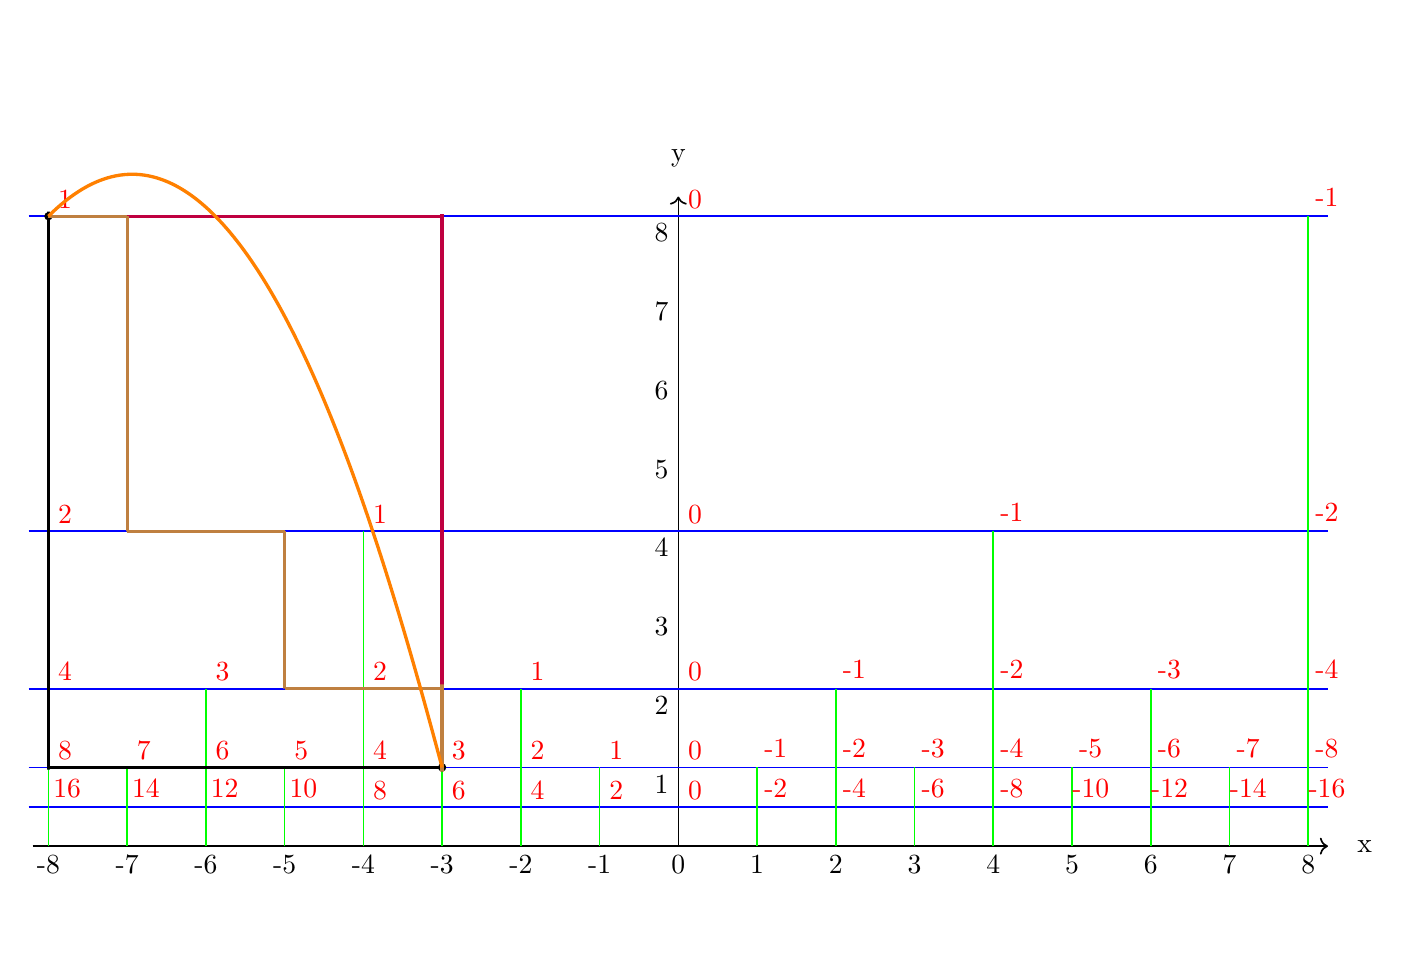
\begin{tikzpicture}
                \draw [black, line width=0.6pt, ->] (0,0) to[out=90,in=270] (0,8.25);
                \node [anchor=south] at (0,8.5) {y};
                \draw [black, line width=0.6pt, ->] (-8.2,0) to[out=0,in=180] (8.25,0);
                \node [anchor=west] at (8.5,0) {x};
                \foreach \x in {-8,-7,-6,-5,-4,-3,-2,-1,0,1,2,3,4,5,6,7,8}
                \node [anchor=north] at (\x,0) {\x};
                \foreach \y in {1,2,3,4,5,6,7,8}
                \node [anchor=45] at (0,\y) {\y};

                \draw [blue, line width=0.6pt] (-8.25,0.5) to[out=0,in=180] (8.25,0.5);
                \draw [blue, line width=0.6pt] (-8.25,1) to[out=0,in=180] (8.25,1);
                \draw [blue, line width=0.6pt] (-8.25,2) to[out=0,in=180] (8.25,2);
                \draw [blue, line width=0.6pt] (-8.25,4) to[out=0,in=180] (8.25,4);
                \draw [blue, line width=0.6pt] (-8.25,8) to[out=0,in=180] (8.25,8);

                \draw [green, line width=0.6pt] (-8,0) to[out=90,in=270] (-8,1);
                \draw [green, line width=0.6pt] (-7,0) to[out=90,in=270] (-7,1);
                \draw [green, line width=0.6pt] (-6,0) to[out=90,in=270] (-6,1);
                \draw [green, line width=0.6pt] (-5,0) to[out=90,in=270] (-5,1);
                \draw [green, line width=0.6pt] (-4,0) to[out=90,in=270] (-4,1);
                \draw [green, line width=0.6pt] (-3,0) to[out=90,in=270] (-3,1);
                \draw [green, line width=0.6pt] (-2,0) to[out=90,in=270] (-2,1);
                \draw [green, line width=0.6pt] (-1,0) to[out=90,in=270] (-1,1);
                \draw [green, line width=0.6pt] (1,0) to[out=90,in=270] (1,1);
                \draw [green, line width=0.6pt] (2,0) to[out=90,in=270] (2,1);
                \draw [green, line width=0.6pt] (3,0) to[out=90,in=270] (3,1);
                \draw [green, line width=0.6pt] (4,0) to[out=90,in=270] (4,1);
                \draw [green, line width=0.6pt] (5,0) to[out=90,in=270] (5,1);
                \draw [green, line width=0.6pt] (6,0) to[out=90,in=270] (6,1);
                \draw [green, line width=0.6pt] (7,0) to[out=90,in=270] (7,1);
                \draw [green, line width=0.6pt] (8,0) to[out=90,in=270] (8,1);

                \draw [green, line width=0.6pt] (-8,1) to[out=90,in=270] (-8,2);
                \draw [green, line width=0.6pt] (-6,1) to[out=90,in=270] (-6,2);
                \draw [green, line width=0.6pt] (-4,1) to[out=90,in=270] (-4,2);
                \draw [green, line width=0.6pt] (-2,1) to[out=90,in=270] (-2,2);
                \draw [green, line width=0.6pt] (2,1) to[out=90,in=270] (2,2);
                \draw [green, line width=0.6pt] (4,1) to[out=90,in=270] (4,2);
                \draw [green, line width=0.6pt] (6,1) to[out=90,in=270] (6,2);
                \draw [green, line width=0.6pt] (8,1) to[out=90,in=270] (8,2);

                \draw [green, line width=0.6pt] (-8,2) to[out=90,in=270] (-8,4);
                \draw [green, line width=0.6pt] (-4,2) to[out=90,in=270] (-4,4);
                \draw [green, line width=0.6pt] (4,2) to[out=90,in=270] (4,4);
                \draw [green, line width=0.6pt] (8,2) to[out=90,in=270] (8,4);

                \draw [green, line width=0.6pt] (-8,4) to[out=90,in=270] (-8,8);
                \draw [green, line width=0.6pt] (8,4) to[out=90,in=270] (8,8);

                \node [anchor=225, red] at (-8,0.5) {16};
                \node [anchor=225, red] at (-7,0.5) {14};
                \node [anchor=225, red] at (-6,0.5) {12};
                \node [anchor=225, red] at (-5,0.5) {10};
                \node [anchor=225, red] at (-4,0.5) {8};
                \node [anchor=225, red] at (-3,0.5) {6};
                \node [anchor=225, red] at (-2,0.5) {4};
                \node [anchor=225, red] at (-1,0.5) {2};
                \node [anchor=225, red] at (0,0.5) {0};
                \node [anchor=225, red] at (1,0.5) {-2};
                \node [anchor=225, red] at (2,0.5) {-4};
                \node [anchor=225, red] at (3,0.5) {-6};
                \node [anchor=225, red] at (4,0.5) {-8};
                \node [anchor=225, red] at (5,0.5) {-10};
                \node [anchor=225, red] at (6,0.5) {-12};
                \node [anchor=225, red] at (7,0.5) {-14};
                \node [anchor=225, red] at (8,0.5) {-16};

                \node [anchor=225, red] at (-8,1) {8};
                \node [anchor=225, red] at (-7,1) {7};
                \node [anchor=225, red] at (-6,1) {6};
                \node [anchor=225, red] at (-5,1) {5};
                \node [anchor=225, red] at (-4,1) {4};
                \node [anchor=225, red] at (-3,1) {3};
                \node [anchor=225, red] at (-2,1) {2};
                \node [anchor=225, red] at (-1,1) {1};
                \node [anchor=225, red] at (0,1) {0};
                \node [anchor=225, red] at (1,1) {-1};
                \node [anchor=225, red] at (2,1) {-2};
                \node [anchor=225, red] at (3,1) {-3};
                \node [anchor=225, red] at (4,1) {-4};
                \node [anchor=225, red] at (5,1) {-5};
                \node [anchor=225, red] at (6,1) {-6};
                \node [anchor=225, red] at (7,1) {-7};
                \node [anchor=225, red] at (8,1) {-8};

                \node [anchor=225, red] at (-8,2) {4};
                \node [anchor=225, red] at (-6,2) {3};
                \node [anchor=225, red] at (-4,2) {2};
                \node [anchor=225, red] at (-2,2) {1};
                \node [anchor=225, red] at (0,2) {0};
                \node [anchor=225, red] at (2,2) {-1};
                \node [anchor=225, red] at (4,2) {-2};
                \node [anchor=225, red] at (6,2) {-3};
                \node [anchor=225, red] at (8,2) {-4};

                \node [anchor=225, red] at (-8,4) {2};
                \node [anchor=225, red] at (-4,4) {1};
                \node [anchor=225, red] at (0,4) {0};
                \node [anchor=225, red] at (4,4) {-1};
                \node [anchor=225, red] at (8,4) {-2};

                \node [anchor=225, red] at (-8,8) {1};
                \node [anchor=225, red] at (0,8) {0};
                \node [anchor=225, red] at (8,8) {-1};

                \node[circle,fill=black,inner sep=1pt,minimum size=3pt] (a) at (-8,8) {};
                \node[circle,fill=black,inner sep=1pt,minimum size=3pt] (b) at (-3,1) {};

                \draw [black, line width=1.2pt] (-8,7.7) to[out=90,in=270] (-8,1.33);
                \draw [black, line width=1.2pt] (-8,1) to[out=0,in=180] (-3,1);

                \draw [purple, line width=1.2pt] (-8,8) to[out=0,in=180] (-3,8);
                \draw [purple, line width=1.2pt] (-3,7.67) to[out=90,in=270] (-3,1.33);

                \draw [brown, line width=1.2pt] (-8,8) to[out=0,in=180] (-7,8);
                \draw [brown, line width=1.2pt] (-7,7.8) to[out=90,in=270] (-7,4.2);
                \draw [brown, line width=1.2pt] (-7,4) to[out=0,in=180] (-5,4);
                \draw [brown, line width=1.2pt] (-5,3.9) to[out=90,in=270] (-5,2.1);
                \draw [brown, line width=1.2pt] (-5,2) to[out=0,in=180] (-3,2);
                \draw [brown, line width=1.2pt] (-3,2) to[out=90,in=270] (-3,1);

                \draw [orange, line width=1.2pt] (-8,8) to[out=45,in=105] (-3,1);

            \end{tikzpicture}
        }
        \label{fig:pathex1}
    \end{figure}
\end{frame}

\begin{frame}
    \frametitle{Arithmetic torsion at scale}
    \begin{columns}
        \begin{column}{0.5\textwidth}
            As the step size increases:

            For a single step:
            \begin{equation}
            (x + 1) \times 2 - (x \times 2 + 1) = 1
            \end{equation}

            For two steps:
            \begin{equation}
            (x + 2) \times 4 - (x \times 4 + 2) = 6
            \end{equation}

            For three steps, the pattern continues:
            \begin{equation}
            (x + 3) \times 8 - (x \times 8 + 3) = 21
            \end{equation}
        \end{column}
        \begin{column}{0.5\textwidth}
            \begin{center}
                \includegraphics[width=1.0\textwidth]{../images/17-area-formula}
            \end{center}
        \end{column}
    \end{columns}
\end{frame}

\begin{frame}
    \frametitle{Eigenfunction of the Laplacian}
    In this setting, \(A = \frac{1}{\mu y}\) and \(B = \frac{1}{\lambda y}\):

    \[
        \Delta f = y^2 \left(\mu^2 \frac{\partial^2 f}{\partial x^2} + \lambda^2 \frac{\partial^2 f}{\partial y^2}\right)
    \]

    For \(f = -\frac{x}{y}\), it follows that

    \[
        \Delta f = - \frac{2 \lambda^2 x}{y} = 2 \lambda^2 f
    \]

    Therefore, \(f = -\frac{x}{y}\) is an eigenfunction of the Laplacian with eigenvalue \(2\lambda^2\).
\end{frame}

\begin{frame}
    \frametitle{When the Alexander polynomial meets the cyclotomic polynomial}
    \begin{itemize}
        \item The figure-eight knot $(4_1)$ has Alexander polynomial $\Delta_{4_1}(t)=t^2-3t+1$.
        \item An AEG path closes precisely when $\Delta_{4_1}(t)=0$.
        \item Cyclotomic polynomials appear in the global arithmetic torsion of the AEG path; for example, $$\tau(a) = \frac{-\Delta_{4_1}(a)(a^2-1)}{a^2}$$.
    \end{itemize}
    \vspace{0.2cm}
    \begin{columns}
        \begin{column}{0.48\textwidth}
            \begin{center}
                \includegraphics[width=0.4\textwidth]{../images/knot_4_1}

                {\small $4_1$ knot}
            \end{center}
        \end{column}
        \begin{column}{0.48\textwidth}
            \begin{center}
                \includegraphics[width=0.6\textwidth]{../images/alexander_4_1}
                
                {\small Alexander-coded path}
            \end{center}
        \end{column}
    \end{columns}
\end{frame}

\begin{frame}
    \frametitle{Binary numeral as flow}
            Examples:
    \begin{center}
         $\left(\frac{3}{2}\right)_{10} = 1.1_{2},\ \left(\frac{7}{4}\right)_{10} = 1.11_{2},\ \left(\frac{21}{8}\right)_{10} = 10.101_{2}.$
        \includegraphics[width=0.7\textwidth]{../images/multiplication}
    \end{center}
\end{frame}

\begin{frame}
    \frametitle{Which complexity does volume measure?}
    It is well known that time and space complexity can trade off against one another.
    \begin{itemize}
        \item Time complexity: number of operations (steps)
        \item Space complexity: memory usage (intermediate results)
    \end{itemize}
    This trade-off suggests a common source of complexity. Which notion of complexity does geometric volume quantify?
\end{frame}

\begin{frame}
    \frametitle{Conclusion: richness from the unified perspective}
    We have shown that:
    \begin{itemize}
        \item Arithmetic expressions can be encoded as geometric flows in the hyperbolic model $\mathfrak{E}_1$; the assignment $a=-x/y$ links computation, geometry, and analysis via the flow equation.
        \item Non-commutativity manifests as arithmetic torsion that scales with step size and organizes paths; analytic structure appears through Laplacian eigenfunctions.
        \item Algebraic invariants such as Alexander and cyclotomic polynomials govern path closure and global torsion, revealing a deep interface between topology and arithmetic.
    \end{itemize}
\end{frame}

%%%%%%%%%%%%%%%%%%%%%%%%%%%%%%%%%%%%%%%%%%%%%%%%%%%%%%%%%%%%%%%%%%%%%%%%%%%%%%%
% Possibility 3: A Neo-Calculus?
%%%%%%%%%%%%%%%%%%%%%%%%%%%%%%%%%%%%%%%%%%%%%%%%%%%%%%%%%%%%%%%%%%%%%%%%%%%%%%%

\section{Malachite: The green stone of renewal}

\begin{frame}
    \frametitle{Malachite: The green stone of renewal}
    \begin{center}
        \Large
        \textbf{A Neo-Calculus?}\newline\newline
        \emph{Can we develop a new calculus that naturally handles mixed operations?}
    \end{center}
\end{frame}

\begin{frame}
    \frametitle{How to describe a change over time?}
    \begin{columns}
        \begin{column}{0.7\textwidth}
            Two methods to describe a small change over time:
            \begin{itemize}
                \item by quantity: adding a small near-zero amount of quantity
                \item by ratio: multiplying a near-unit ratio
            \end{itemize}
            Traditional calculus is based on the first method, Riemann integral is additive.
            We can use functions $\exp$ and $\log$ to convert between the two methods.
        \end{column}
        \begin{column}{0.3\textwidth}
            \begin{figure}[ht]\centering
            \resizebox{1.0\textwidth}{!}{\includegraphics{../images/fluxions}}
            \caption{Method of Fluxions}
            \end{figure}
        \end{column}
    \end{columns}
\end{frame}

\begin{frame}
    \frametitle{Product integration}
    \begin{columns}
            \begin{column}{0.3\textwidth}
                \begin{figure}[ht]\centering
                \resizebox{1.0\textwidth}{!}{\includegraphics{../images/vito_volterra}}
                \caption{Vito Volterra}
                \end{figure}
            \end{column}
            \begin{column}{0.7\textwidth}
            Matrix-valued non-commutative derivative and integration, left and right
            \begin{itemize}
                \item $\frac{d}{dx} A(x) = \lim_{\Delta x \to 0} \frac{A(x + \Delta x) A^{-1}(x) - I}{\Delta x}$
                \item $A(x) \frac{d}{dx} = \lim_{\Delta x \to 0} \frac{A^{-1}(x) A(x + \Delta x) - I}{\Delta x}$
                \item $\prod_{a}^{b} (I + A(x) dx) = \lim_{\nu(P) \to 0} \prod_{i=m}^{1}(I + A(\xi_i))$
                \item $(I + A(x) dx) \prod_{a}^{b}  = \lim_{\nu(P) \to 0} \prod_{i=1}^{m}(I + A(\xi_i))$
            \end{itemize}
            An interesting formula connect product integration and normal additive integration
            $\prod_a^b (I + A(x) dx) = I + \int_a^b A(x) dx + \int_a^b \int_a^x A(x) A(y) dy dx + \cdots$
            \end{column}
    \end{columns}
\end{frame}

\begin{frame}
    \frametitle{How about mixing up additive and multiplicative steps?}
    The additive calculus provide a closed set over polynomials over differential and integral operators.
    \begin{itemize}
        \item $\frac{d}{dx} p(x) = q(x)$
        \item $\int p(x) dx = q(x) + C$
    \end{itemize}
    This is the fundamental source of power series, Laurent series and approximation theory.
    \newline\newline
    Problem: How about mixing additive and multiplicative steps up in one process?
    \newline\newline
    Directions:
    \begin{itemize}
        \item We need handle functions other than constants in arithmetic expressions.
        \item We need expand polynomials to another closed set over differential and integral operators.
    \end{itemize}
\end{frame}

\begin{frame}
    \frametitle{A contact structure}
    Consider $(u,v,a)\in\mathbb{R}^3$ with constants $\mu,\lambda$.
    \[
      \omega := \mu\,du + \lambda a\,dv,\qquad \alpha := da - \omega
    \]
    Key properties:
    \begin{itemize}
      \item Contact:
      \[
        d\omega=\lambda\,da\wedge dv,\quad d\alpha=-d\omega,\quad
        \alpha\wedge d\alpha=\mu\lambda\,du\wedge da\wedge dv\neq 0
      \]
      so $\alpha$ is a contact form when $\mu\lambda\neq 0$.
      \item Reeb field and distribution:
      \[
        R=-(1/\mu)\,\partial_u,\qquad \mathcal{H}:=\ker\alpha
      \]
      \item Horizontal lifts (basis of $\mathcal{H}$):
      \[
        D_u:=\partial_u+\mu\,\partial_a,\qquad
        D_v:=\partial_v+\lambda a\,\partial_a,\qquad \alpha(D_u)=\alpha(D_v)=0
      \]
      \item Normal units: with $\tilde u=\mu u,\ \tilde v=\lambda v$,
      \[
        \alpha=da-d\tilde u-a\,d\tilde v
      \]
    \end{itemize}
\end{frame}

\begin{frame}
    \frametitle{Calculus over the contact structure: I}
    The expression differential $\delta$ is defined by
    \[
      \delta a=\omega,\qquad \delta u=du,\qquad \delta v=dv,
    \]
    and for any $F(u,v,a)$
    \[
      \delta F = dF - (\partial_a F)\,\alpha
      = (D_uF)\,du + (D_vF)\,dv,
    \]
    where
    \[
      D_uF=F_u+\mu F_a,\qquad D_vF=F_v+\lambda a F_a,\qquad
      D_\theta=\cos\theta\,D_u+\sin\theta\,D_v.
    \]
    Chain rules:
    \[
      \delta\Phi(a)=\Phi'(a)\,\omega,\qquad
      \delta F(E_1,E_2)=\partial_1F\,\delta E_1+\partial_2F\,\delta E_2.
    \]
\end{frame}

\begin{frame}
    \frametitle{Calculus over the contact structure: II}
    Curvature and non-commutativity:
    \[
      [D_u,D_v]=\mu\lambda\,\partial_a,\qquad
      \delta^2F=\mu\lambda(\partial_a F)\,du\wedge dv,\qquad
      \delta^2 a=\mu\lambda\,du\wedge dv.
    \]
    Compatibility and circulation:
    \[
      (d\omega)^*\big|_{\alpha=0}=\mu\lambda\,du\wedge dv,\qquad
      \oint_{\partial\Sigma}\omega=\iint_\Sigma d\omega=\mu\lambda\iint_\Sigma du\wedge dv.
    \]
    Quick rules:
    \[
      \delta(a^n)=n a^{n-1}\omega,\quad
      \delta(\ln a)=\tfrac{\omega}{a},\quad
      \delta(e^a)=e^a\omega,\quad
      \delta(\sin a)=\cos a\,\omega,\quad
      \delta(\cos a)=-\sin a\,\omega.
    \]
    Rectification and flow:
    \[
      y=\arcsin\!\left(\tfrac{\lambda a}{\mu}\right),\quad \|\nabla y\|=\lambda,\quad
      \frac{da}{ds}=D_\theta a=\mu\cos\theta+\lambda a\sin\theta.
    \]
\end{frame}

\begin{frame}
  \frametitle{Extending polynomials: the affine–Appell basis}
  Normal units: $\tilde u=\mu u,\ \tilde v=\lambda v$. Define scaled powers
  \[
    B_n(a,v):=e^{-n\tilde v}a^n\quad(n\in\mathbb{N}).
  \]
  Let
  \[
    \mathcal{B}:=\Big\{\sum_{n=0}^N P_n(u,v,e^{\tilde v})\,B_n(a,v)\ \text{(finite)}\Big\}.
  \]
  \textbf{Closure Theorem.} $\mathcal{B}$ is closed under the mixed calculus generated by
  \[
    D_u=\partial_u+\mu\,\partial_a,\qquad D_v=\partial_v+\lambda a\,\partial_a.
  \]
  Rules:
  \[
    D_u(PB_n)=(\partial_u P)B_n+\mu n\,e^{-\tilde v}P\,B_{n-1},\quad
    D_v(PB_n)=(\partial_v P)B_n.
  \]
\end{frame}

\begin{frame}
  \frametitle{Antiderivatives and a finite upward sweep}
  If $P$ is independent of $u$,
  \[
    D_u^{-1}\!\big(P(v,e^{\tilde v})\,B_n\big)=\frac{e^{\tilde v}P(v,e^{\tilde v})}{\mu(n+1)}\,B_{n+1}.
  \]
  In general, define $Q^{(0)}_n=\dfrac{e^{\tilde v}}{\mu(n+1)}P_n$ and set $G^{(0)}=\sum_n Q^{(0)}_nB_{n+1}$.
  Then $F-\!D_uG^{(0)}=-\sum_n(\partial_uQ^{(0)}_n)B_{n+1}$. Repeat finitely many times.
  \vspace{0.6em}

  \textbf{Example.} For $F=a^3e^{\lambda v}=e^{4\tilde v}B_3$,
  \[
    D_u^{-1}F=\frac{e^{\tilde v}}{4\mu}B_4=\frac{e^{\lambda v}}{4\mu}a^4,\quad
    D_u\!\left(\frac{e^{\lambda v}}{4\mu}a^4\right)=a^3e^{\lambda v}.
  \]
\end{frame}

%%%%%%%%%%%%%%%%%%%%%%%%%%%%%%%%%%%%%%%%%%%%%%%%%%%%%%%%%%%%%%%%%%%%%%%%%%%%%%%
% Possibility 4: A New Atlas for Complex Analysis?
%%%%%%%%%%%%%%%%%%%%%%%%%%%%%%%%%%%%%%%%%%%%%%%%%%%%%%%%%%%%%%%%%%%%%%%%%%%%%%%

\section{Quartz: The white stone of clarity}

\begin{frame}
    \frametitle{Quartz: The white stone of clarity}
    \begin{center}
        \Large
        \textbf{A New Atlas for Complex Analysis?}
        \newline\newline
        \emph{Is complex analysis a special case of a more general theory?}
    \end{center}
\end{frame}


%%%%%%%%%%%%%%%%%%%%%%%%%%%%%%%%%%%%%%%%%%%%%%%%%%%%%%%%%%%%%%%%%%%%%%%%%%%%%%%
% Possibility 5: A Key to the Non-linear Maze?
%%%%%%%%%%%%%%%%%%%%%%%%%%%%%%%%%%%%%%%%%%%%%%%%%%%%%%%%%%%%%%%%%%%%%%%%%%%%%%%

\section{Obsidian: The black stone of depth}

\begin{frame}
    \frametitle{Obsidian: The black stone of depth}
    \begin{center}
        \Large
        \textbf{A Key to the Non-linear Maze?}
        \newline\newline
        \emph{Can AEG help us navigate the complexities of non-linear systems?}
    \end{center}
\end{frame}

%%%%%%%%%%%%%%%%%%%%%%%%%%%%%%%%%%%%%%%%%%%%%%%%%%%%%%%%%%%%%%%%%%%%%%%%%%%%%%%
% Final Thoughts
%%%%%%%%%%%%%%%%%%%%%%%%%%%%%%%%%%%%%%%%%%%%%%%%%%%%%%%%%%%%%%%%%%%%%%%%%%%%%%%

\section{Final Thoughts}


\end{document}
